\documentclass[a4paper, 10pt]{article}

\usepackage[english, russian]{babel}
\usepackage[T2A]{fontenc}
\usepackage[utf8]{inputenc}
\usepackage{mathtext}
\usepackage{amsfonts}
\usepackage{ amssymb }
\usepackage{amsmath}
\usepackage{graphics}
\usepackage{graphicx}
\usepackage{wrapfig}
\usepackage{geometry}
\usepackage{float}
\usepackage{hyperref}
\geometry{
        a4paper,
        total={170mm, 257mm},
        left=20mm,
        top=10mm}

\title{Лабораторная работа 3.5.1. Изучение плазмы газового разряда в неоне.}
\author{Балдин Виктор}
\date{\today}
\begin{document}
        \maketitle
        \section*{Теория}
        \subsection*{Плазма}

        Из-за теплового движения в плазме электроны могут смещаться относительно ионов и образовывать неоднородности. В этих неоднородностях возникает электрическое поле, которое стремится восстановить баланс, из-за чего происходят колебания с частотой
        \[w_p = \sqrt{\frac{4\pi n_e e^2}{m_e}}\]
        За характерное время колебаний электроны за счет теплового движения смещаются на
        \[r_D \sim \frac{v_e}{w_p} = \sqrt{\frac{kT_e}{4\pi n_e e^2}}\]
        $r_D$ - дебаевский радиус, $k$ - константа Больцмана.\\
        Если поместить в плазму пробную (допустим, положительную) частицу, то электроны будут скапливаться около этой частицы, экранируя её поле. Потенциал точечного заряда будет иметь в плазме следующий вид:
        \[\varphi(r) = \frac{q}{r}e^{-\frac{r}{r_D}}\]
        где $r_D = \sqrt{\dfrac{kT_e}{4\pi n e^2}}$ -- \textit{радиус Дебая в случае равновесной плазмы}. Если температуры электронов и ионов сильно отличаются, то следует определять отдельно величину радиуса экранирования для электронов и для ионов. Итоговый радиус будет
        \[r_D = (r_{De}^{-2} + r_{Di}^{-2})^{-1/2}\]
        То есть если $T_i \ll T_e$, то $r_D \approx r_{Di}$
        \subsection*{Одиночный зонд}
        При внесении в плазму уединённого проводника -- \textit{зонда} -- с потенциалом, изначально равным потенциалу точки плазмы, в которую его помещают, на него поступают токи электроннов и ионов:
        \begin{equation}
                \begin{array}{c}
                        I_{e0} = \dfrac{n \langle v_e \rangle}{4}eS,\\
                        I_{i0} = \dfrac{n \langle v_i \rangle}{4}eS,
                \end{array}
        \end{equation}
        где $\langle v_e \rangle$ и $\langle v_i \rangle$ -- средние скорости электронов и ионов, $S$ -- площадь зонда, $n$ -- плотность электронов и ионов. Скорости электронов много больше скорости ионов, поэтому $I_{i0} \ll I_{e0}$. Зонд будет заряжаться до некоторого равновестного напряжения $-U_f$ -- \textit{плавающего потенциала}.\\
        В равновесии ионный ток мало меняется, а электронный имеет вид
        $$
        I_e = I_0 \exp\left( -\dfrac{eU_f}{kT_e} \right).
        $$
        Будем подавать потенциал $U_\text{з}$ на зонд и снимать значение зондового тока $I_\text{з}$. Максимальное значение тока $I_{e\text{н}}$ -- электронный ток насыщения, а минимальное $I_{i\text{н}}$ -- ионный ток насыщения. Значение из эмпирической формулы Бомона:
        \begin{equation}
                I_{i\text{н}} = 0.4 neS \sqrt{\dfrac{2kT_e}{m_i}}.
        \end{equation}

        Электронный ток насыщения можно определить по тепловому движению:
        \[I_{e\text{н}} = \frac{n_eS}{4}\sqrt{\frac{8kT}{\pi m_e}}\]
        \subsection*{Двойной зонд}
        Двойной зонд -- система из двух одинаковых зондов, расположенных на небольшом расстоянии друг от друга, между которыми создаётся разность потенциалов, меньшая $U_f$. Рассчитаем ток между ними вблизи $I=0$. При небольших разностях потенциалов ионные токи на оба зонда близки к току насыщения и компенсируют друг друга, а значит величина результирующего тока полностью связана с разностью электронных токов. Пусть потенциалы на зондах
        $$
        U_1 = -U_f + \Delta U_1,
        $$
        $$
        U_2 = -U_f + \Delta U_2.
        $$
        Между зондами $U = U_2 - U_1 = \Delta U_2 - \Delta U_1$.
        Через первый электрод
        \begin{equation}
                I_1 = I_{i\text{н}} + I_{e1} = I_{i\text{н}} - \dfrac{1}{4}neS\langle v_e\rangle \exp\left(-\dfrac{eU_f}{kT_e}\right)\exp\left(\dfrac{e\Delta U_1}{kT_e}\right)=I_{i\text{н}}\left(1 - \exp\left( \dfrac{e\Delta U_1}{kT_e} \right)\right).
        \end{equation}
        Аналогично через второй получим
        \begin{equation}
                I_2 = I_{i\text{н}}\left(1 - \exp\left( \dfrac{e\Delta U_2}{kT_e} \right)\right)
        \end{equation}

        Из $(7)$ и $(8)$ с учётом последовательного соединение зондов ($I_1 = -I_2 = I)$:
        $$
        \Delta U_1= \dfrac{kT_e}{e}\text{ln}\left(1 - \dfrac{I}{I_{i\text{н}}}\right)
        $$
        $$
        \Delta U_2= \dfrac{kT_e}{e}\text{ln}\left(1 + \dfrac{I}{I_{i\text{н}}}\right)
        $$

        Тогда итоговые формулы для разности потенциалов и тока

        \begin{equation}
                U = \dfrac{kT_e}{e}\text{ln}\dfrac{1 - I/I_{i\text{н}}}{1 + I/I_{i\text{н}}}, \ \
                I = I_{i\text{н}} \text{th}\dfrac{eU}{2kT_e} + AU.
                \label{tok}
        \end{equation}

        \begin{figure}[h!]
                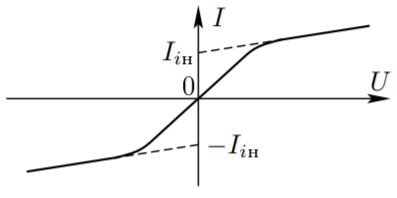
\includegraphics[scale=0.8]{4.png}
        \end{figure}
        Зависимость выглядит примерно так.
        С учетом \ref{tok} можно выразить асимптоты графика:
        \begin{equation}
                I = I_{i\text{нас}} + AU,\ I = -I_{i\text{нас}} + AU
        \end{equation}
        Наклон в нуле принимает вид:
        \begin{equation}
          \frac{dI}{dU} = I_{i\text{нас}} \frac{e}{2kT_e} + A
        \end{equation}

        \section*{Описание установки}
        \begin{center}
                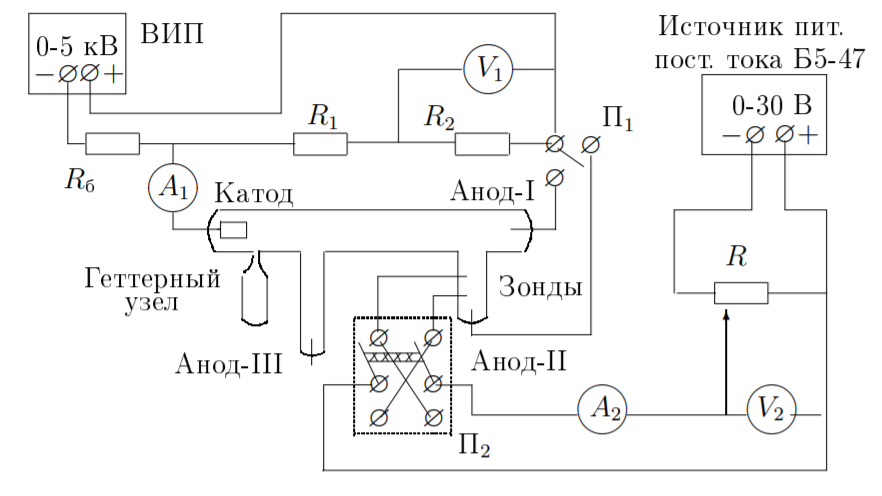
\includegraphics[scale=0.9]{1.png}
        \end{center}
        Стеклянная газоразрядная трубка имеет холодный (ненакаливаемый) полый катод, три анода и \textit{геттерный} узел -- стеклянный баллон, на внутреннюю повехность которого напылена газопоглощающая плёнка (\textit{геттер}). Трубка наполнена изотопом неона $^22$Ne при давлении 2 мм рт. ст. Катод и один из анодом (I и II) с помощью переключателя $\Pi_1$ подключается через балластный резистор $R_\text{б}$ ($\approx 450$ кОм) к регулируемому ВИП с выкодным напряжением до 5 кВ.\\
        При подключении к ВИП анода-I между ним и катодом возникает газовый разряд. Ток разряда измеряется миллиамперметром $A_1$, а падение напряжения на разрядной трубке -- цифровым вольтметром $V_1$, подключённым к трубке черезе высокоомный (25 МОм) делитель напряжения с коэффициентом $(R_1+R_2)/R_2 = 10$.\\
        При подключении к ВИП анода-II разряд возникает в пространстве между катодом и анодом-II, где находятся двойной зонд, используемый для диагностики плазмы положительного столба. Зонды изготовлены из молибденовой проволоки диаметром $d = 0.2$ мм и имеют длину $l = 5.2$ мм. Они подключены к источнику питания GPS через потенциометр $R$. Переключатель $\Pi_2$ позволяет изменять полярность напряжения на зондах. Величина напряжения на зондах изменяеься с помощью дискретного переключателя <<$V$>> выходного напряжения источника питания и потенциометра $R$, а измеряется цифровым вольтметром $V_2$. Для измерения зондового тока используется мультиметр $A_2$.

        \section*{Ход работы}
        Измеряем напряжение зажигания в лампе: $U_{\text{заж}} = 99\pm5 $ В.\\
        Снимаем ВАХ газового разряда. Результаты представлены в таблице.
        % \begin{table}[h!]
        % 	\centering
        % 	\begin{tabular}{|c|c|c|c|c|c|c|c|c|c|}
        % 		\hline
        % 		$I$, мА & 0,506 & 0,991 & 1,505 & 2,014 & 2,506 & 3,004 & 3,507 & 3,999 & 4,518 \\ \hline
        % 		$U$, В & 35,07 & 33,50 & 30,86 & 29,47 & 28,48 & 27,54 & 26,90 & 26,98 & 27,25 \\ \hline
        % 	\end{tabular}
        % \end{table}

        Построим ВАХ и определим максимальное дифференциальное сопротивление разряда $R_{\text{диф}} = \frac{dU}{dI}$. Оно будет соответствовать участку с минимальным (по модулю) наклоном графика $I(U)$:

        \begin{figure}[h!]
        	\centering
        	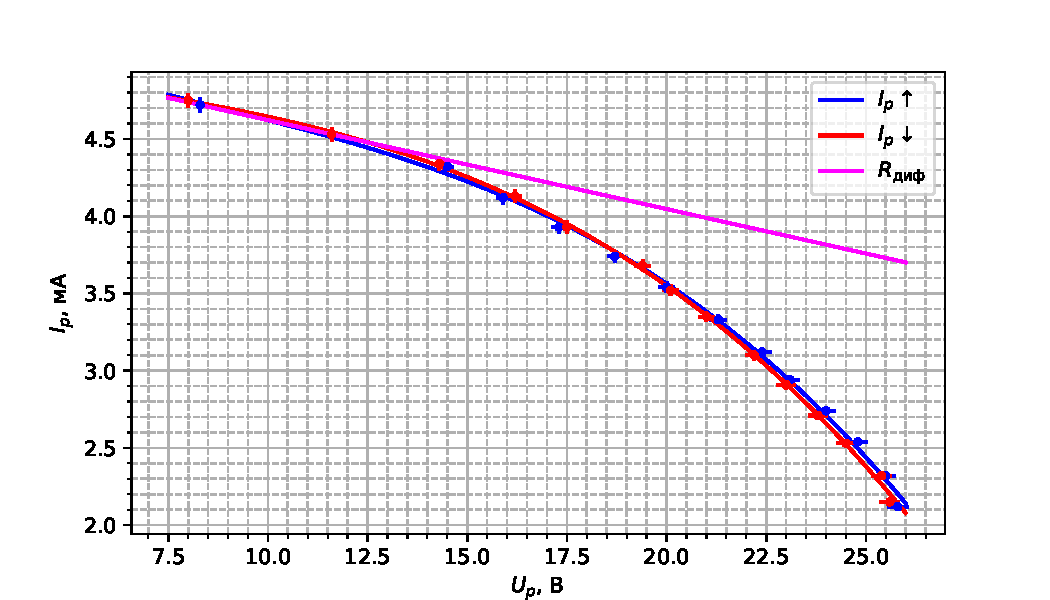
\includegraphics[width = \textwidth]{vah.pdf}
        	\caption{ВАХ газового разряда в неоне}
        \end{figure}
        В схеме напряжение снимается с делителя напряжений с коэффициентом 10, поэтому $R_{\text{диф}} = -17 \pm 6$ кОм. Наш график соответствует участку поднормального тлеющего разряда (см. приложение к лабораторной работе).

        % \newpage
        С помощью вольтмертра $V_2$ и амперметра $A_2$ снимем ВАХ двойного зонда $I_2 = f(U_2)$ при фиксированного токе разряда $I_p$ в трубке в диапозоне $-25 \div 25$ В, процессе измерений меняя полярность зонда при нулевом токе. Измерения проведём для $I_p = 4.0$ мА, $I_p = 3.0$ мА  и $I_p = 2.3$ мА.

        \begin{figure}[h!]
        	\centering
        	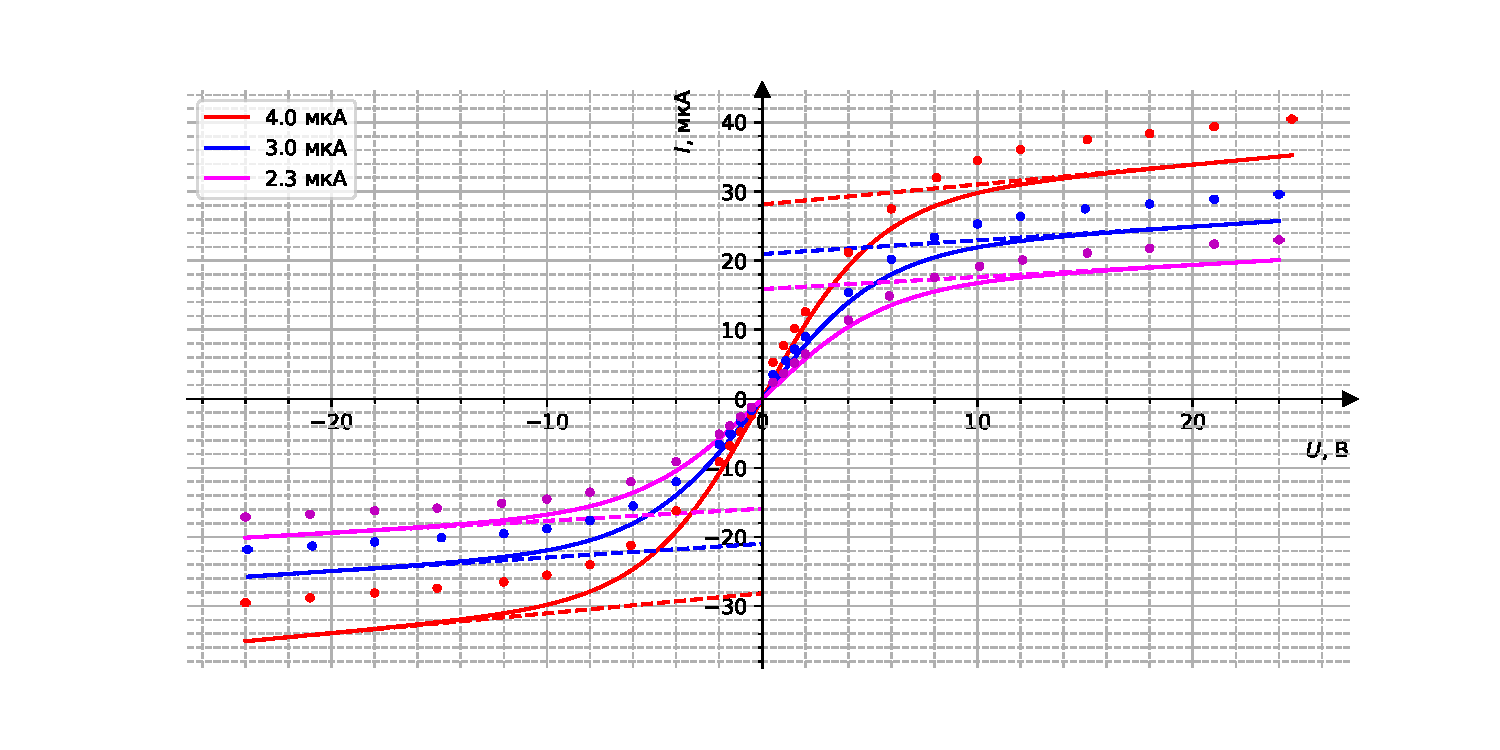
\includegraphics[width = \textwidth]{zond.pdf}
          \caption{Зондовые характеристики}
        \end{figure}

        Видно, что чем меньше ток, тем менее крутая кривая получается. Проанализируем графики по отдельности, чтобы найти их наклон в начале и пересечение асимптот с осью ординат. Данные будем заносить в таблицу. Ионный ток насыщения определим через асимптоты, затем по наклону кривой в точке $U = 0$ найдем концентрацию электронов в плазме.

      \begin{table}[h!]
      \begin{tabular}{|c|c|c|c|c|c|c|c|}
      \hline
      $I_p$, мА & $T_e$, $10^4$ K & $n_e$, $10^{14}$ м$^{-3}$ & $\omega_p$, $10^3$ рад/с & $r_{D_e}$, $10^{-3}$ м & $r_D$, $10^{-4}$ м & $N_D$, $10^5$ & $\alpha$, $10^{-7}$ \\ \hline
      4.0 & $ 3.1 \pm  0.8$ & $1.4 \pm 0.3$ & $7.0 \pm 0.8$ & $10 \pm 2$ & $10 \pm 1$ & $5.2 \pm 0.6$ & $5.2 \pm 1.2$ \\ \hline
      3.0 & $ 3.1 \pm  0.8$ & $1.0 \pm 0.2$ & $6.0 \pm 0.7$ & $11 \pm 2$ & $11 \pm 1$ & $6.0 \pm 0.7$ & $3.8 \pm 0.9$ \\ \hline
      2.3 & $ 3.3 \pm  0.8$ & $0.8 \pm 0.2$ & $5.2 \pm 0.6$ & $14 \pm 3$ & $13 \pm 1$ & $7.0 \pm 0.8$ & $2.8 \pm 0.7$ \\ \hline
      \end{tabular}

      \end{table}


      По данным таблицы видно что $N_D \gg 1 \Rightarrow$ плазму можно с хорошей точностью считать идеальной.

        % \begin{table}[h!]
        % 	\centering
        % 	\begin{tabular}{|c|c|c|c|c|c|c|}
        % 		\hline
        % 		$I_p$, мА  & $T_e$, $10^3$ К & $kT_e$, эВ & $n_e$, $10^{16}$ м$^{-3}$ & $\omega_p$, $10^9 \frac{\text{рад}}{c}$ & $r_{De}$, $10^{-3}$ cм & $r_D, 10^{-4}$ см  \\ \hline
        % 		5.02   & $65.5\pm 4.5$ & $5.6 \pm 0.4$ & $5.17 \pm 0.37$                     & $12.8\pm 0.5$                   & $7.76\pm 0.28$    &   $5.25 \pm 0.19$            \\ \hline
        % 		3.02   & $66.0\pm 3.3$ & $5.7 \pm 0.3$ &$3.95\pm 0.21$                     & $11.2\pm 0.3$                    & $8.92\pm 0.24$    &  $6.01 \pm 0.16$               \\ \hline
        % 		1.52   & $50.6	\pm 1.2$ &$4.4 \pm 0.1$ &$2.08\pm 0.03$                    & $8.1\pm 0.1$                     & $10.75 \pm 0.07$  &  $8.28 \pm 0.06$                 \\ \hline
        % 	\end{tabular}
        % 	\caption{Результаты вычислений}
        % \end{table}

        % \begin{figure}
        % 	\centering
        % 	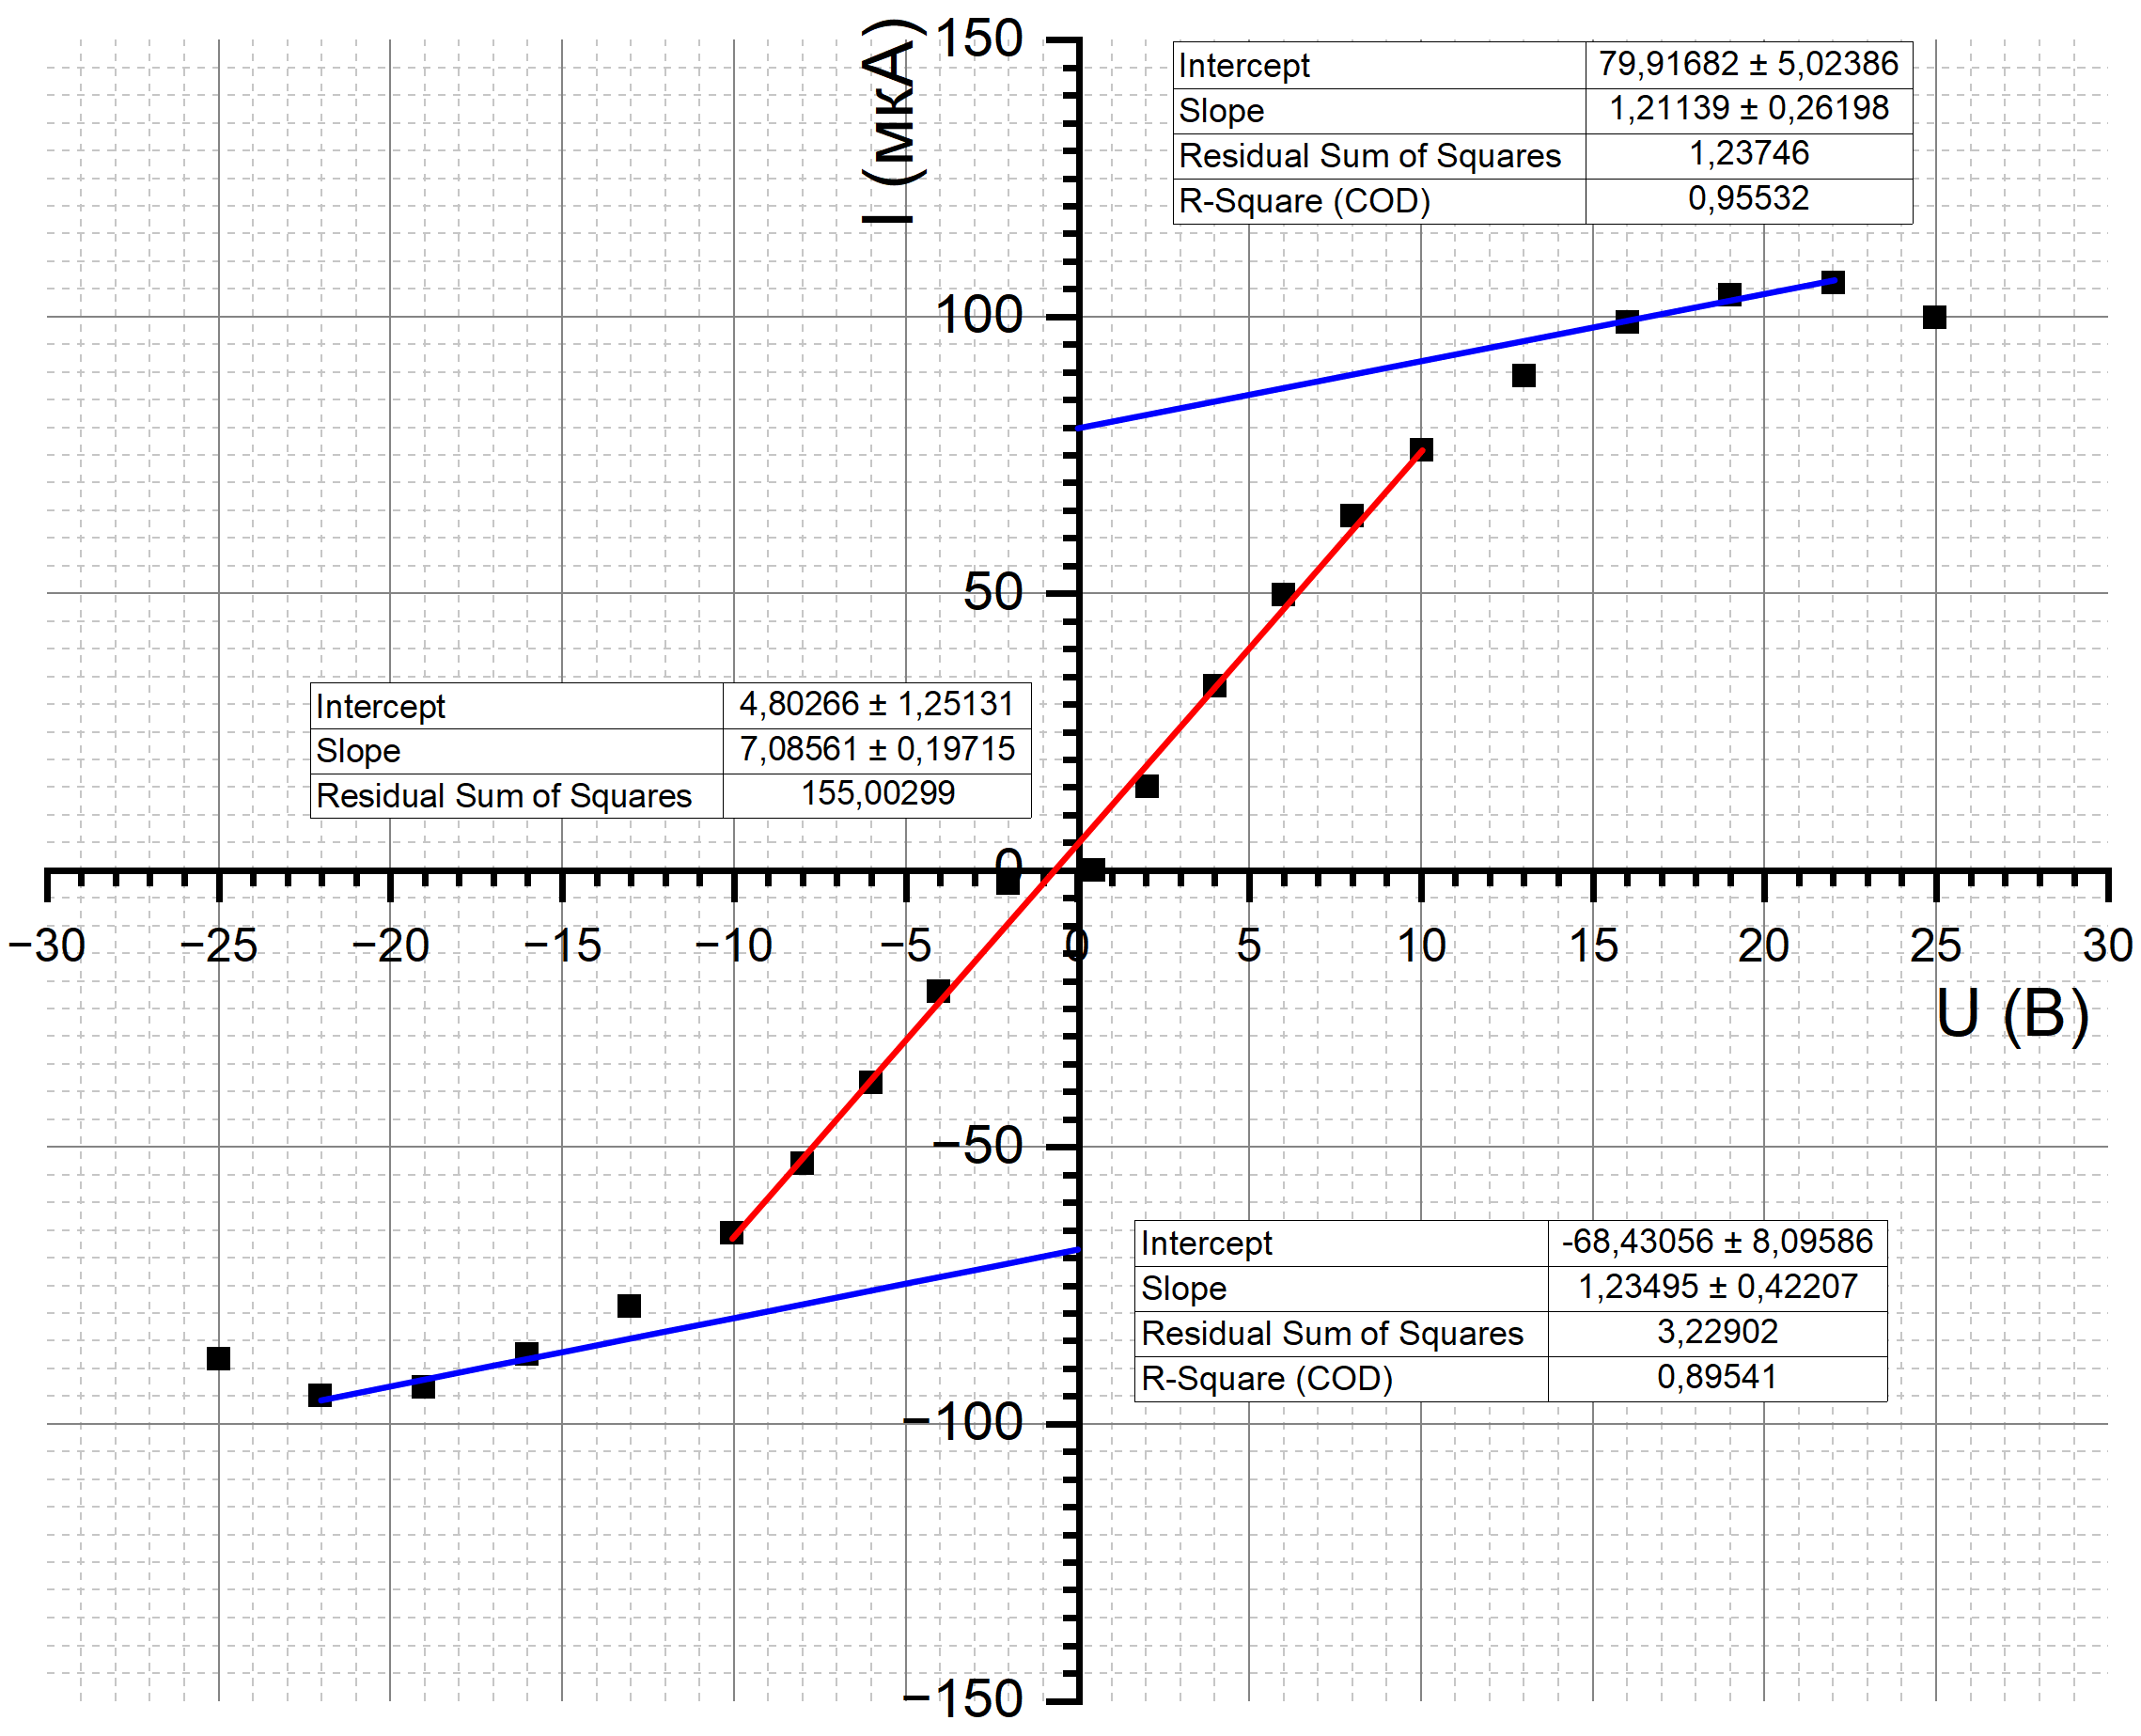
\includegraphics[width = 0.87\textwidth, height = 0.45\textheight]{5mA}
        % 	\caption{ВАХ зонда при $I_p = 5,02$ мА}
        % \end{figure}

        % \begin{figure}
        % 	\centering
        % 	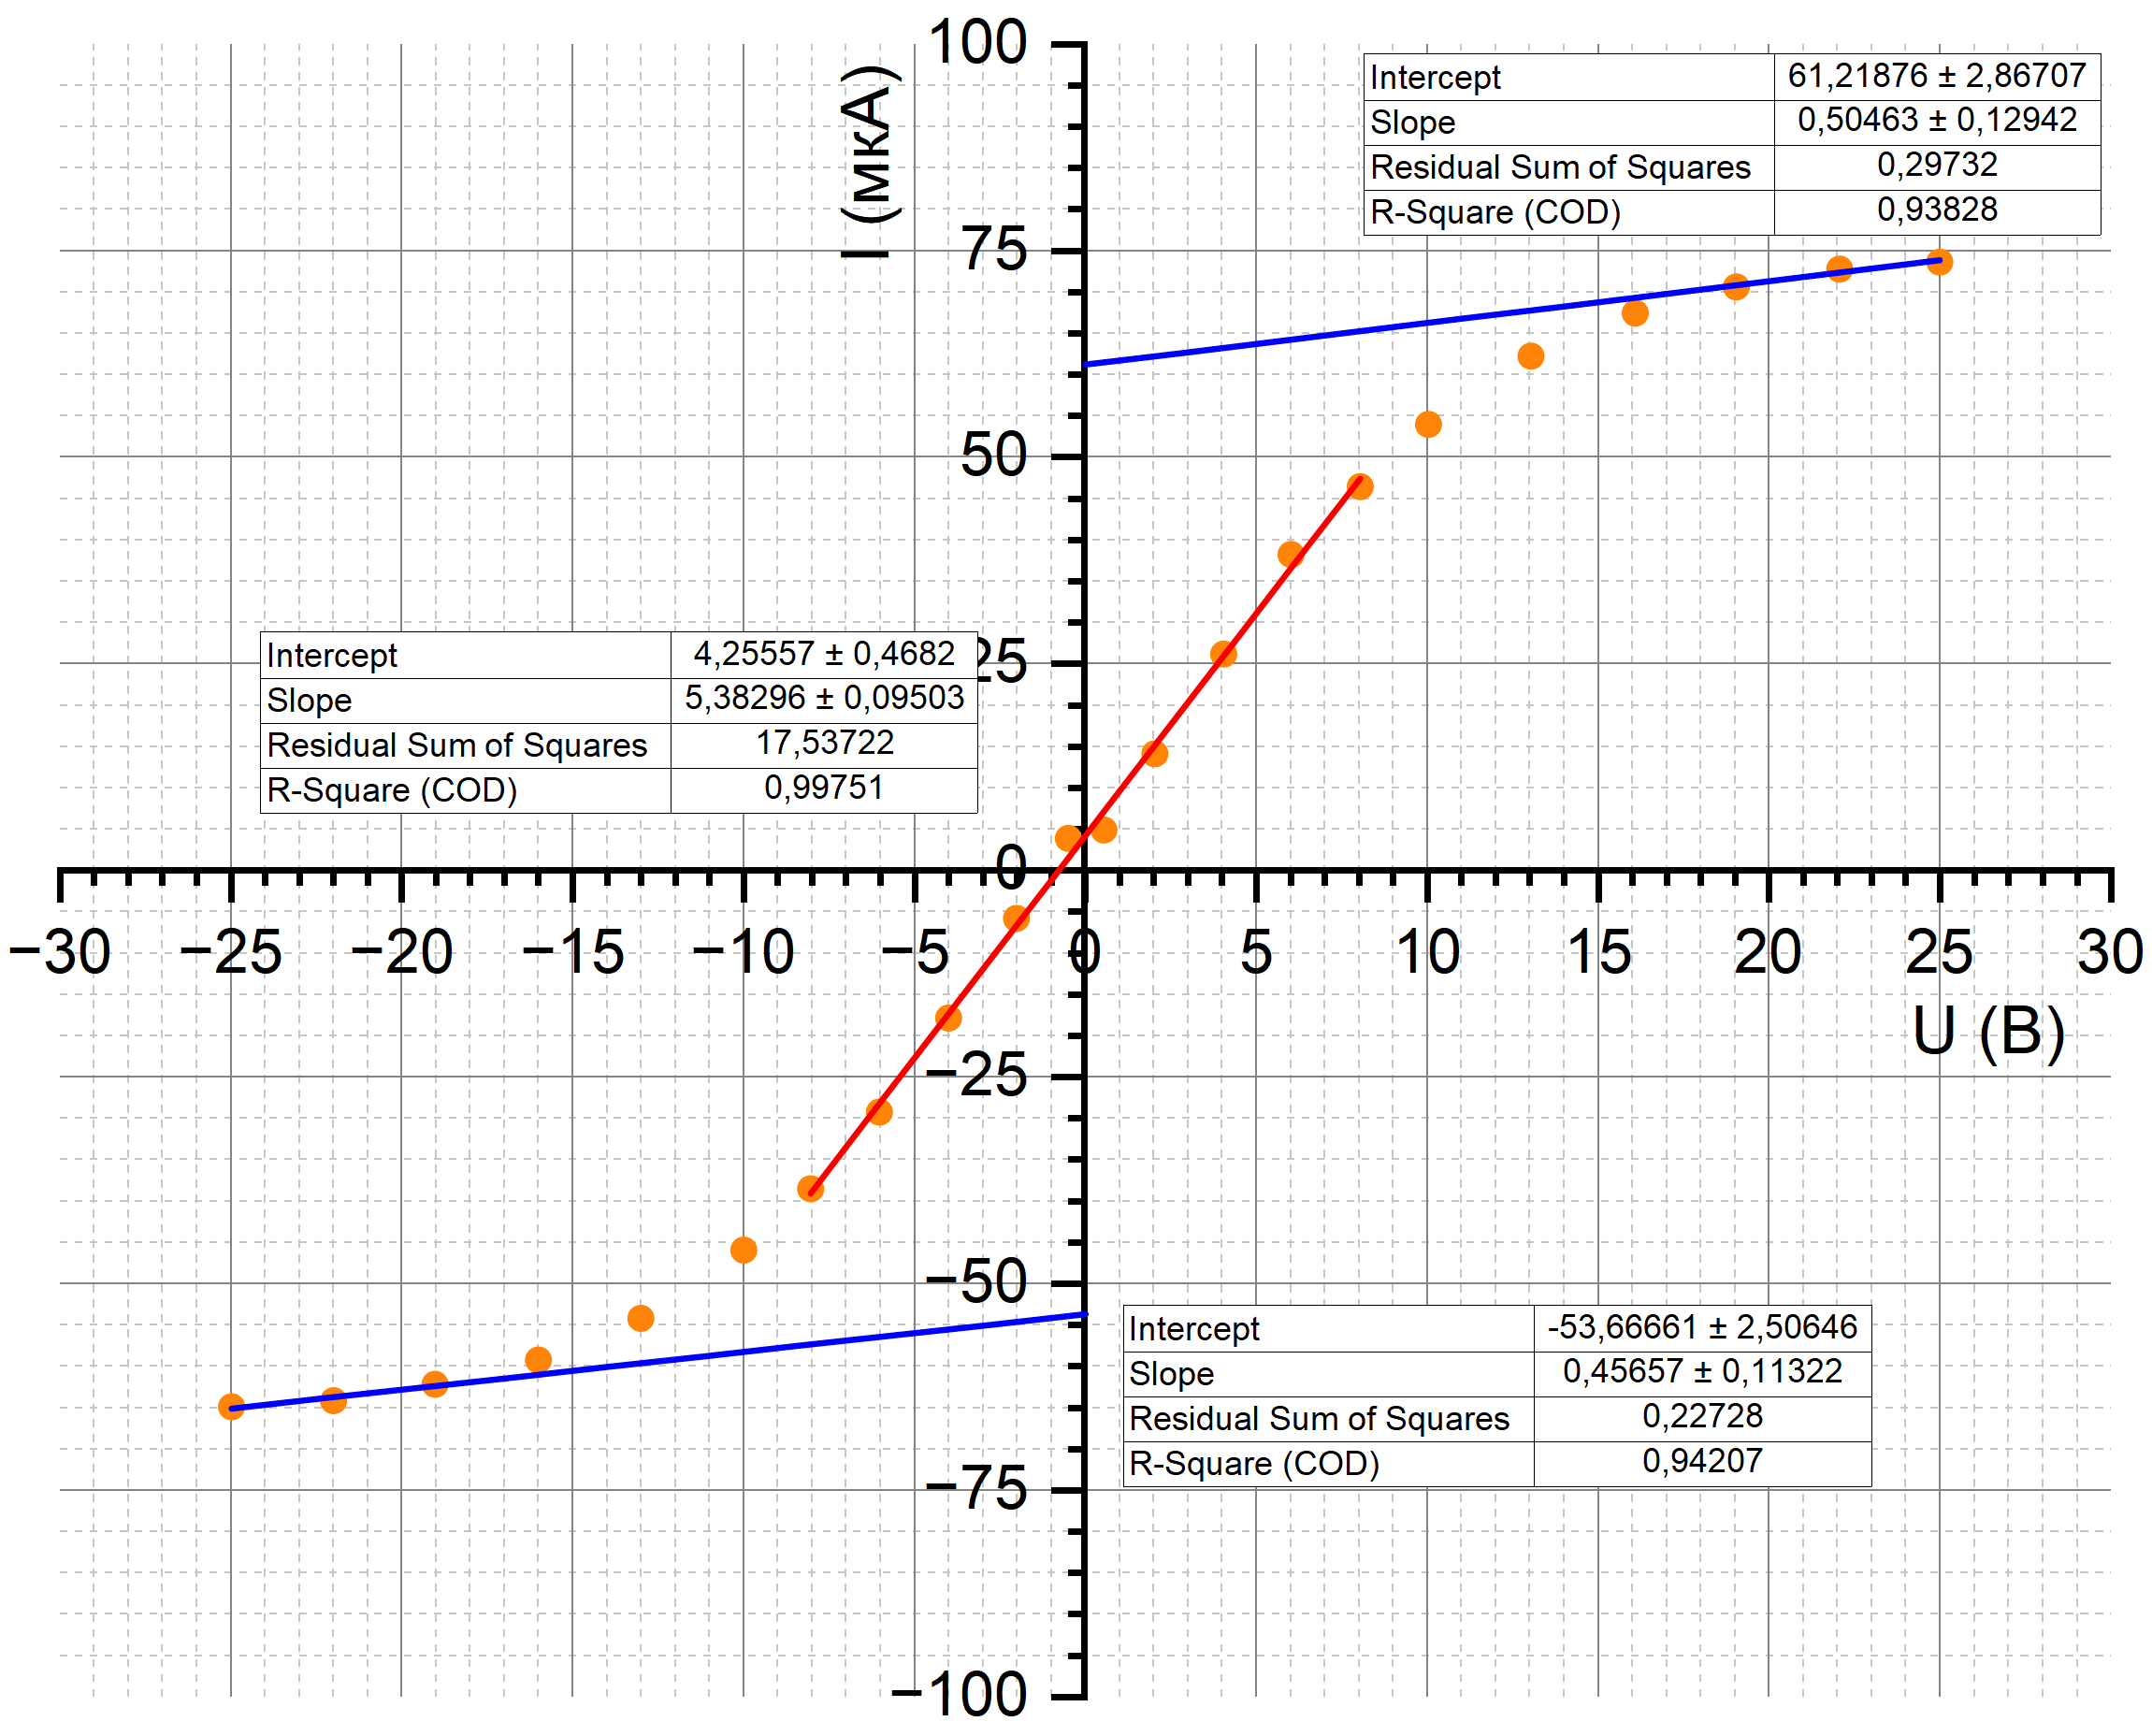
\includegraphics[width = 0.87\textwidth, height = 0.45\textheight]{3mA}
        % 	\caption{ВАХ зонда при $I_p = 3,02$ мА}
        % \end{figure}

        % \begin{figure}[h!]
        % 	\centering
        % 	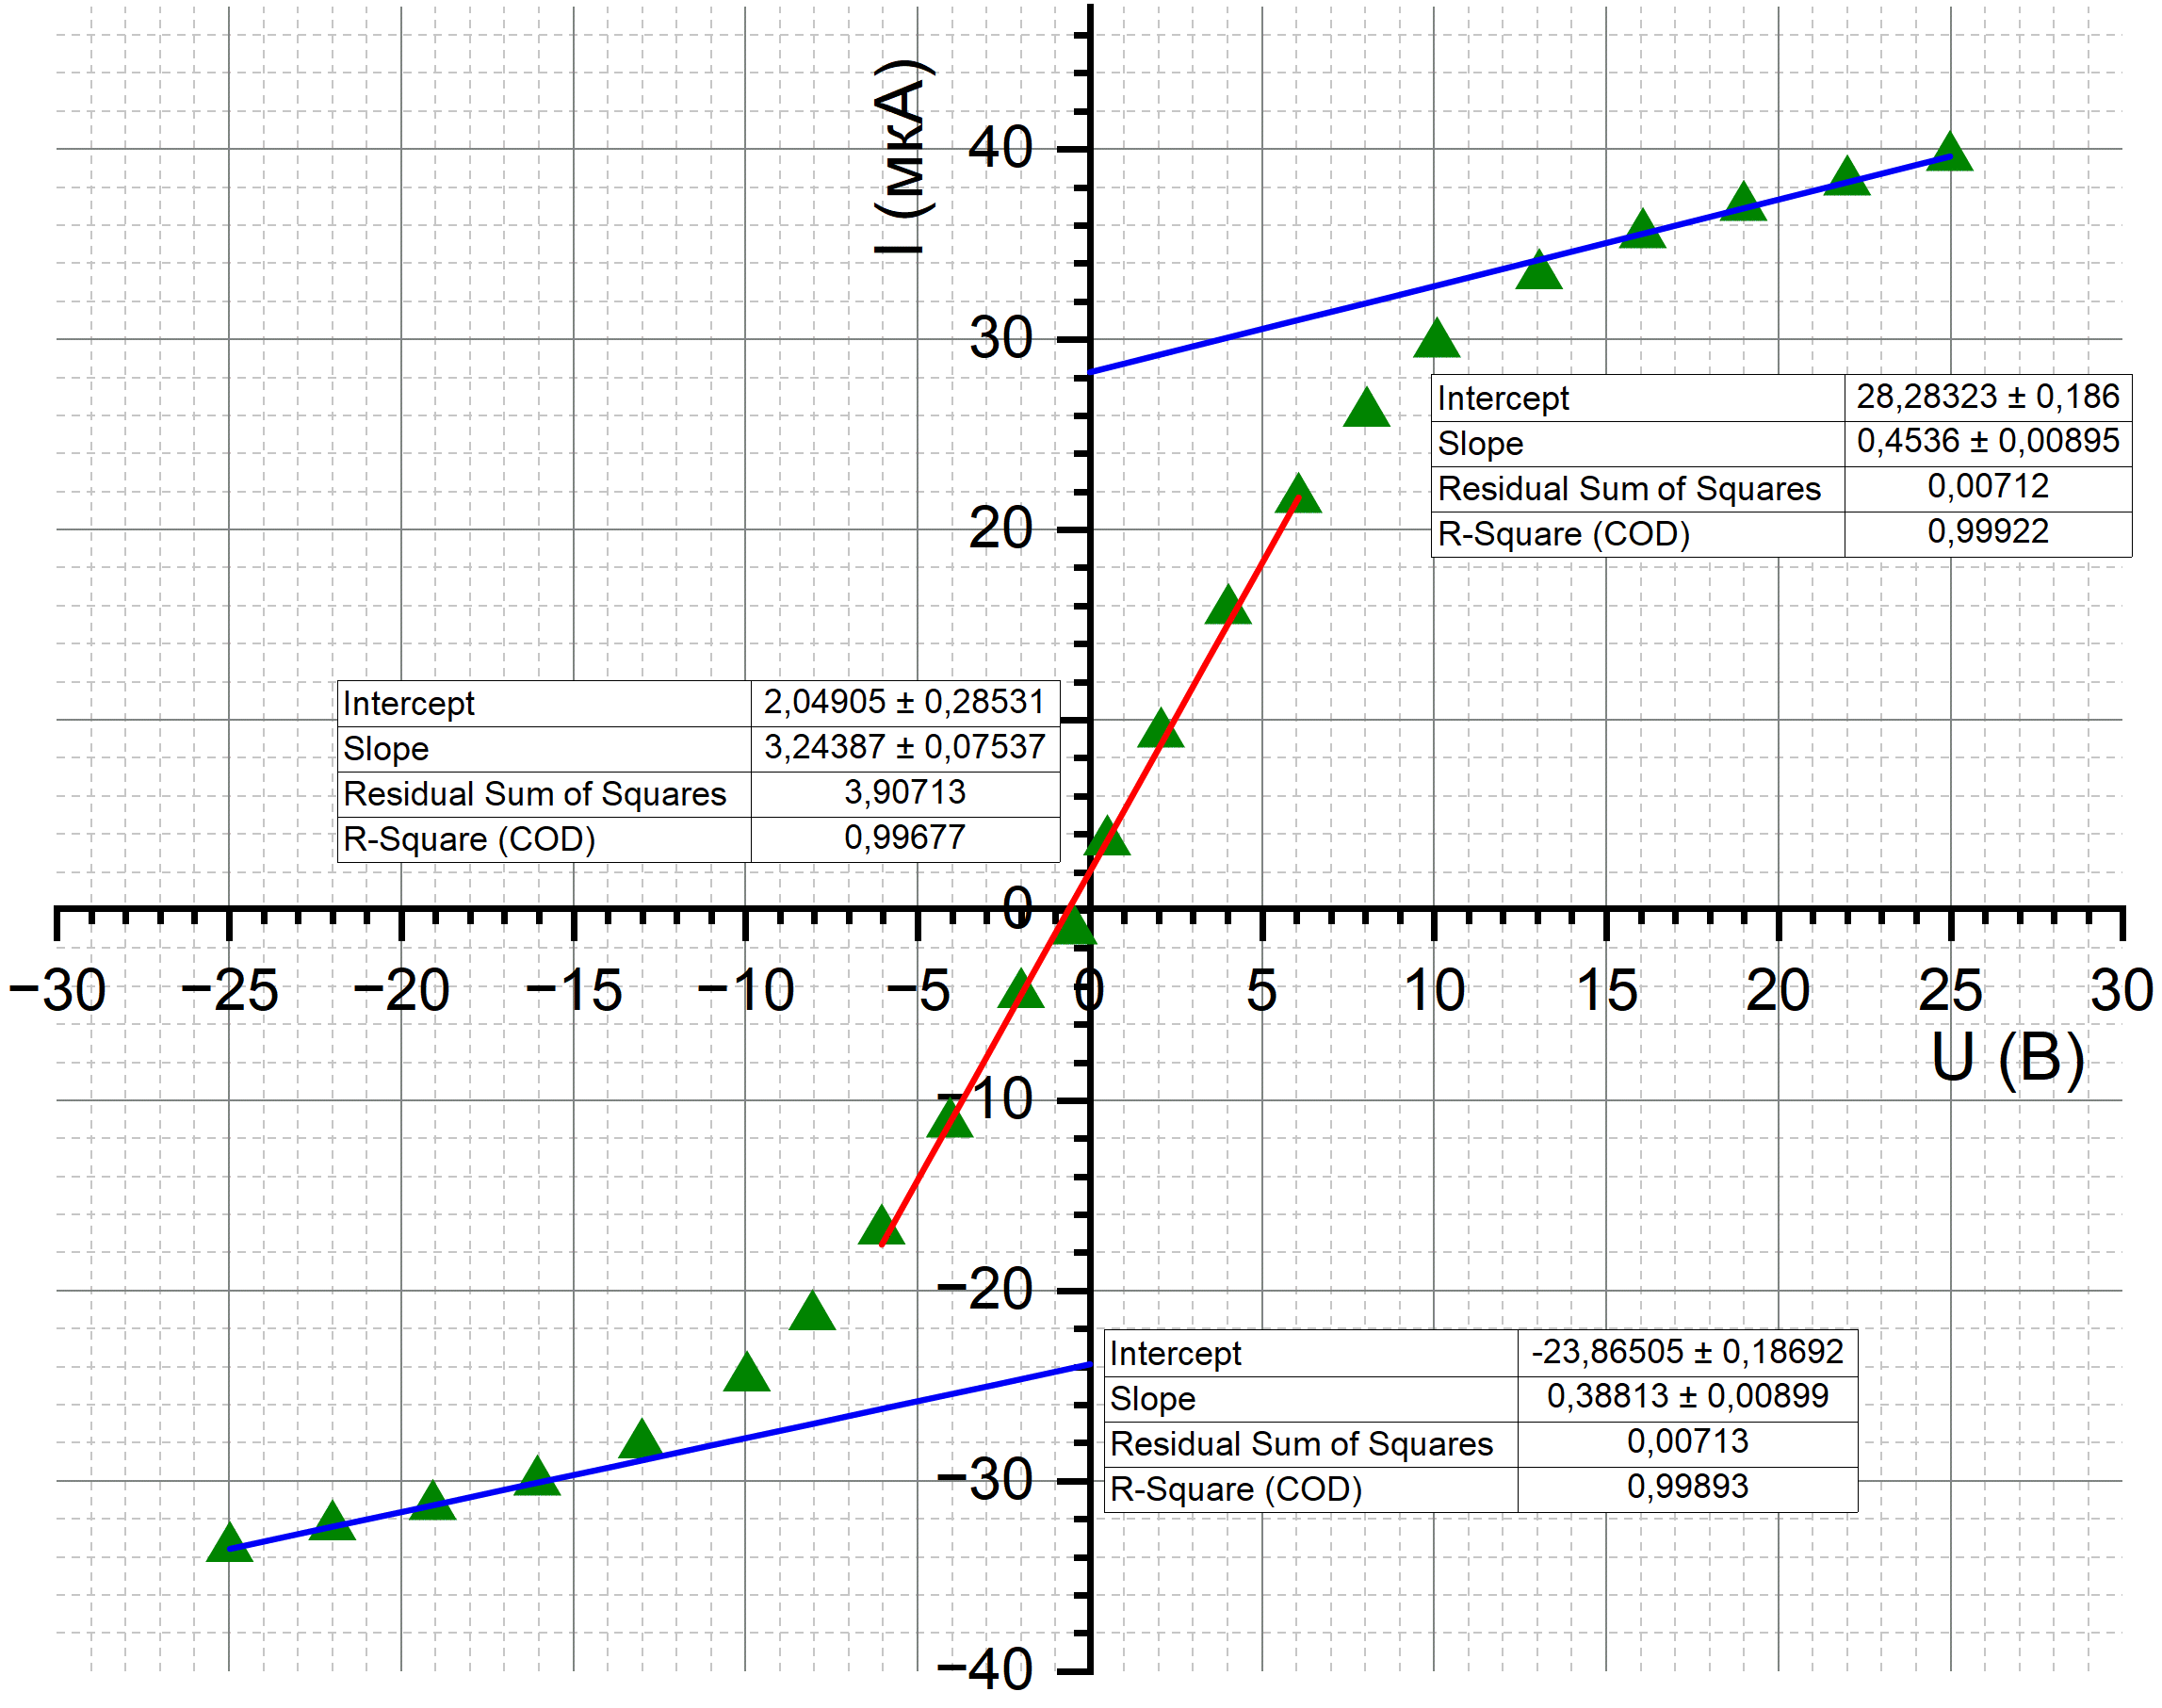
\includegraphics[width = \textwidth]{1,5mA}
        % 	\caption{ВАХ зонда при $I_p = 1,52$ мА}
        % \end{figure}
        % \newpage
        % $r_D$ рассчитываем в предположении, что $T_i \ll T_e, \ T_i \approx 300 K$.

        % Степень ионизации $\alpha$ рассчитаем из условия, что $P \approx 2$ торр. $\alpha = \dfrac{n_i}{n}$, где $P = nkT_i$
        % \begin{table}[h!]
        % 	\centering
        % 	\begin{tabular}{|c|c|c|}
        % 		\hline
        % 		$I_p$, мА & $N_D$ & $\alpha, 10^{-7}$ \\ \hline
        % 		5.02 & $31.4 \pm 4.1 $ & $8.03 \pm 0.58$ \\ \hline
        % 		3.02 & $35.9 \pm 3.4$ & $6.13 \pm 0.33$ \\ \hline
        % 		1.52 & $49.4 \pm 1.2$ & $3.23 \pm 0.04$ \\ \hline
        % 	\end{tabular}
        % 	\caption{Результаты вычислений}
        % \end{table}

        % Относительные погрешности вычисленных величин показаны в процентах в таблице :
        % \begin{table}[h!]
        % 	\centering
        % 	\begin{tabular}{|c|c|c|c|c|c|c|c|c|}
        % 		\hline
        % 		$I_p$,мА & $T_e$ & $kT_e$ & $n_e$ & $\omega_p$ & $r_{De}$ & $r_D$ & $N_D$ & $\alpha$ \\ \hline
        % 		 5.02 & 6.9 & 6.9 & 7.2 & 3.6 & 3.6 & 3.6 & 12.9 & 7.2 \\ \hline
        % 		 3.02 & 5.0 & 5.0 & 5.3 & 2.7 & 2.7 & 2.7 & 9.6 & 5.3 \\ \hline
        % 		 1.52 & 2.4 & 2.4 & 1.4 & 0.7 & 0.7 & 0.7 &2.5 & 1.4 \\ \hline
        % 	\end{tabular}
        % 	\caption{Относительные погрешности величин в процентах}
        % \end{table}

        \newpage
        Построим графики $T_e(I_p)$ и $n(I_p)$:

        \begin{figure}[h!]
        	\centering
        	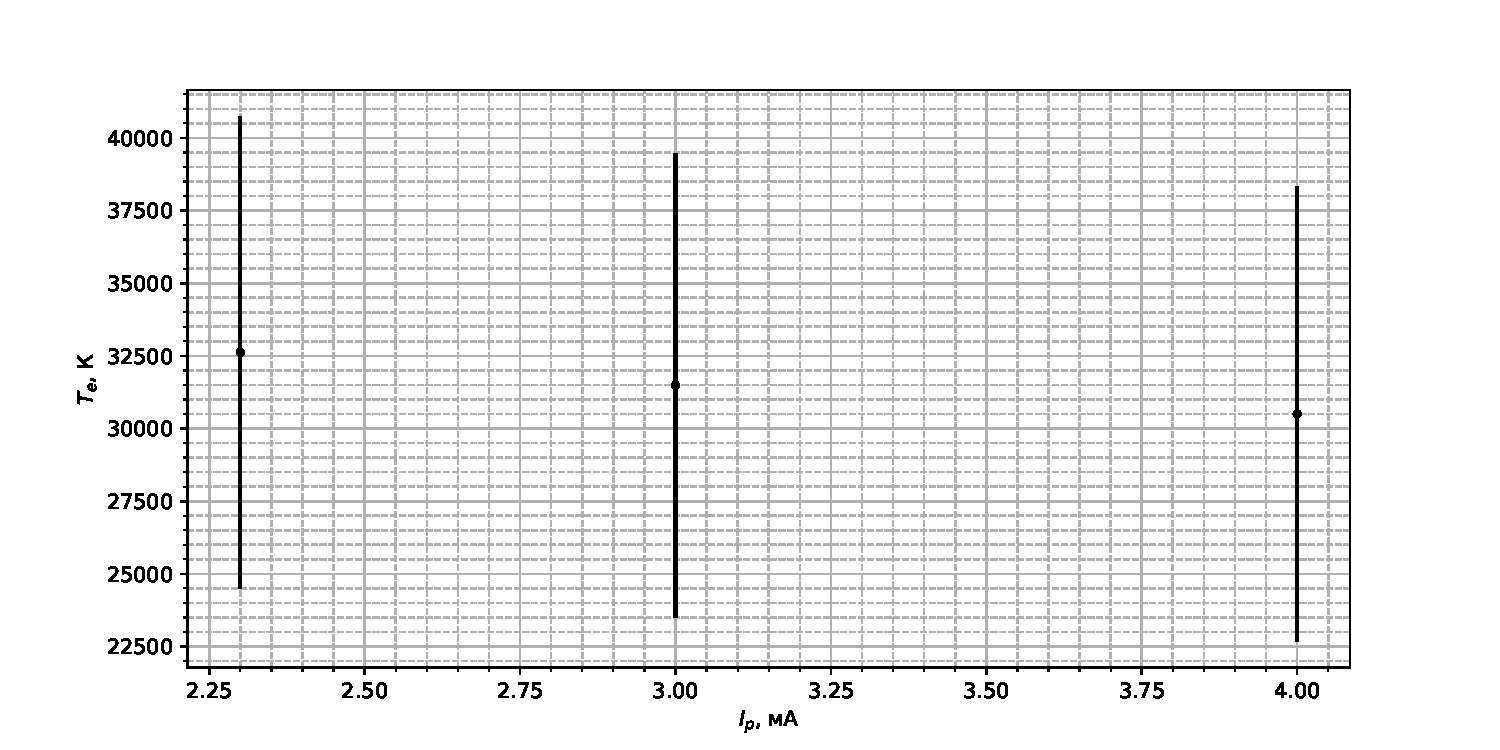
\includegraphics[width = \textwidth]{t.pdf}
        	\caption{Зависимость $T_e(I_p)$}
        \end{figure}
        \begin{figure}[h!]
        	\centering
        	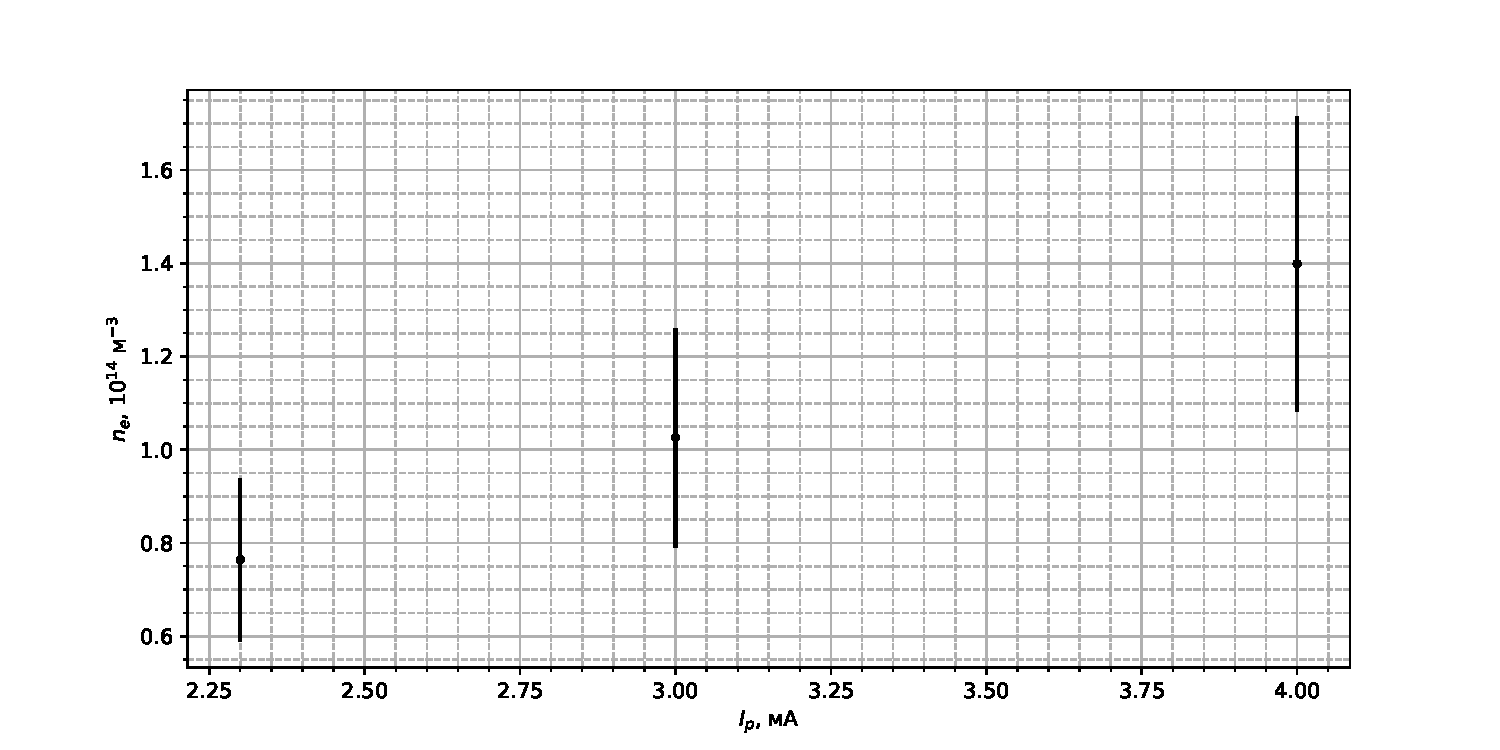
\includegraphics[width = \textwidth]{n.pdf}
        	\caption{Зависимость $n(I_p)$}
        \end{figure}

        Очевидно, что из-за больших погрешностей эксперимента судить о характере $T_e(I_p)$ невозможно,
        но зависимость $n(I_p)$ возрастает при повышении тока, потому что больше молекул газа ионизируется, так как выше электрическое поле, выше скорость электронов и больше столкновений.

        % \newpage
        % В обоих случая в пределах погрешности зависимости можно назвать возрастающими. Концентрация электронов возрастает Температура электронов возрастает, но зависимость не близка к линейной.

        \newpage
        \section*{Вывод}
        В данной лабораторной работе мы исследовали состояние плазмы в тлеющем газовом разряде c помощью двойного зонда. Полученные результаты сходятся с указанными в лабораторной работе по порядку. Плазму в тлеющем разряде можно с хорошей точностью назвать идеальной, так как $N_D \gg 1$.

\end{document}